
\section{ARP}

\subsection{Скриншоты}

\begin{center}

    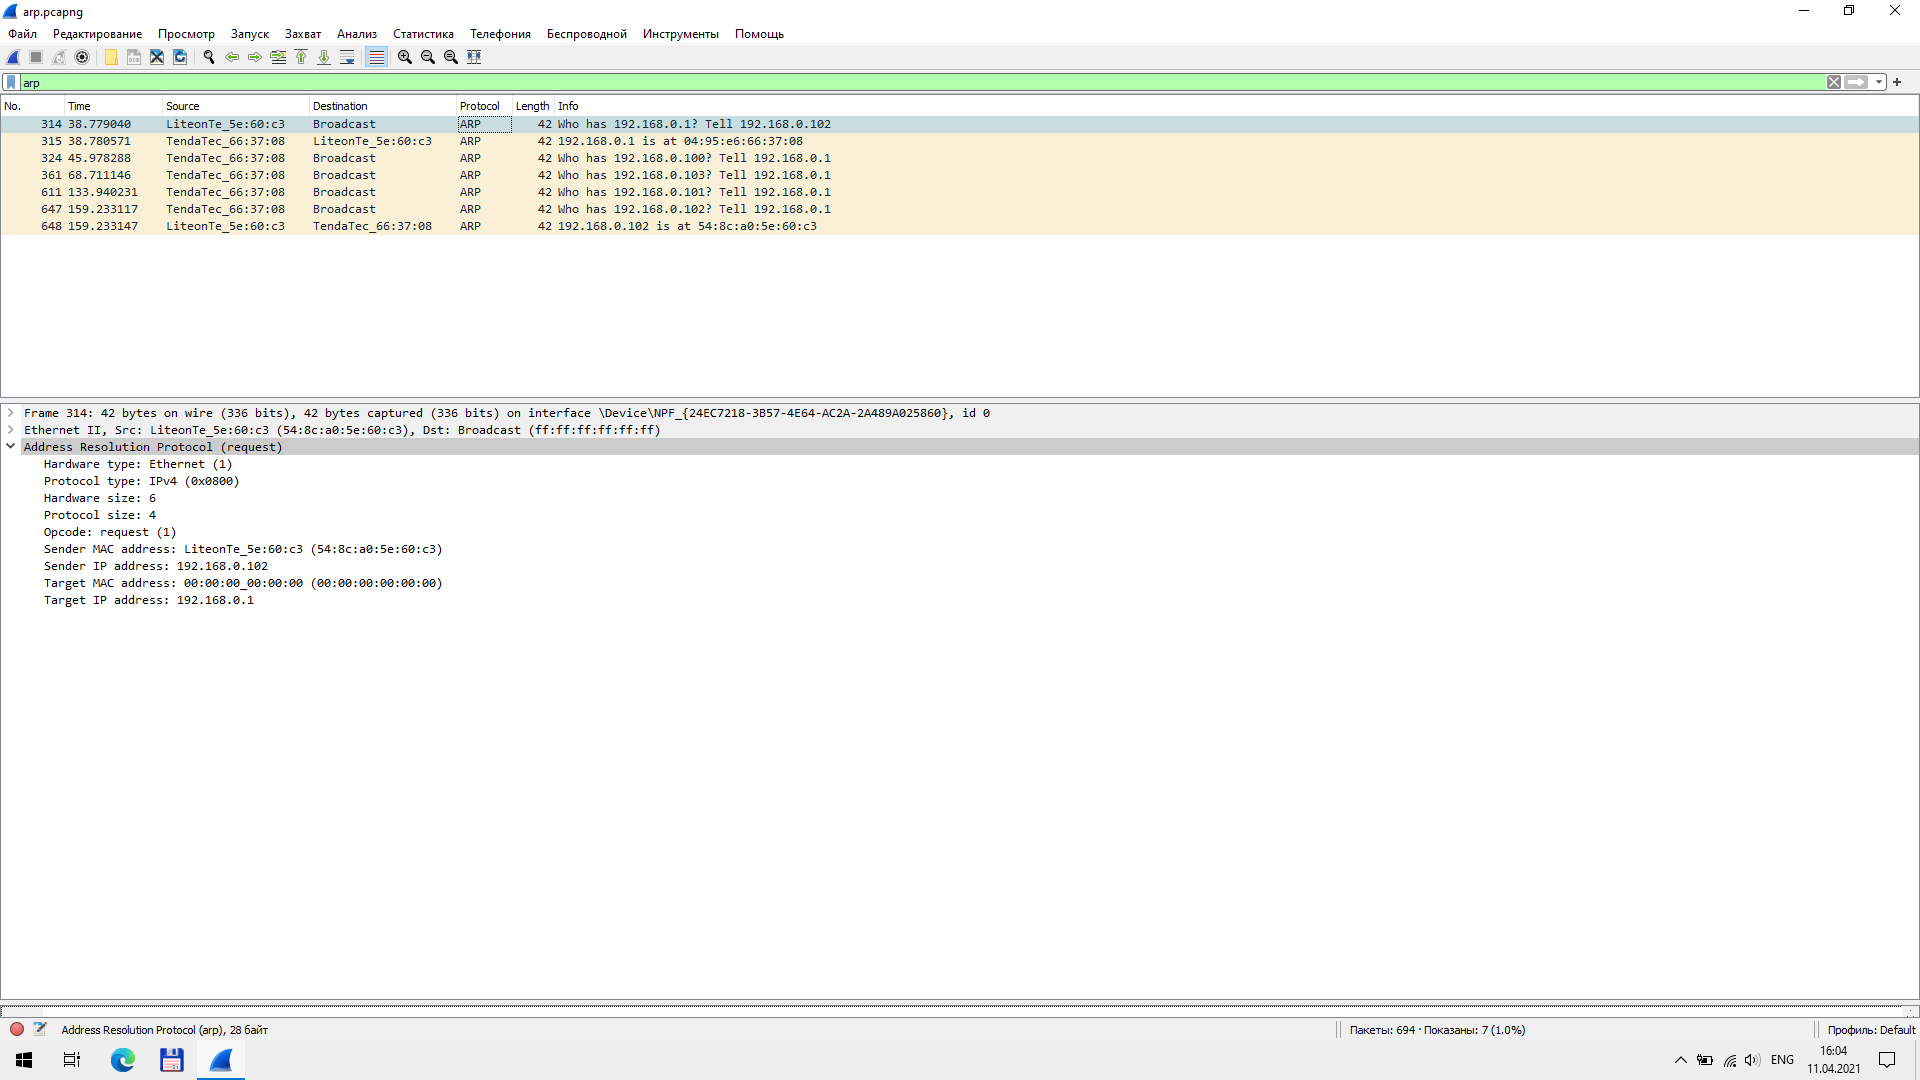
\includegraphics[width=\textwidth]{screenshots/arp_request_1}

    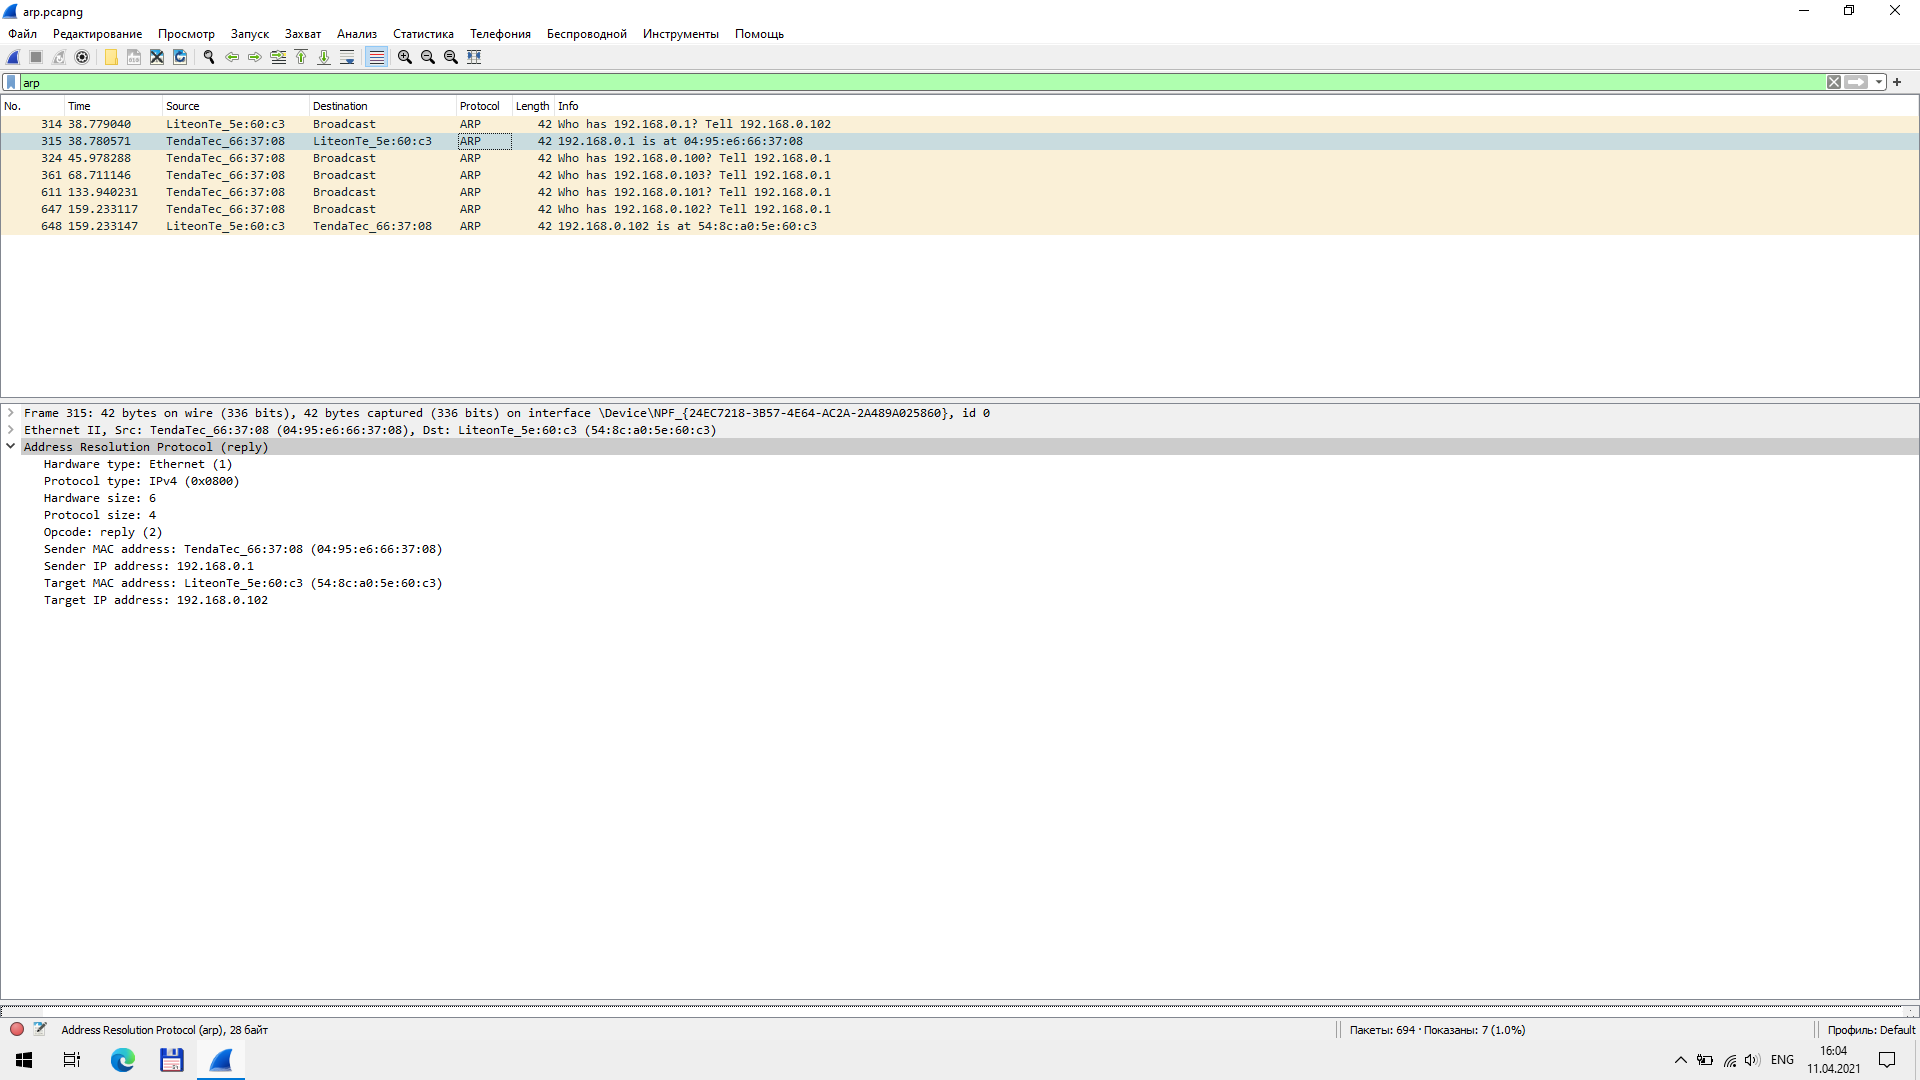
\includegraphics[width=\textwidth]{screenshots/arp_response_1}

    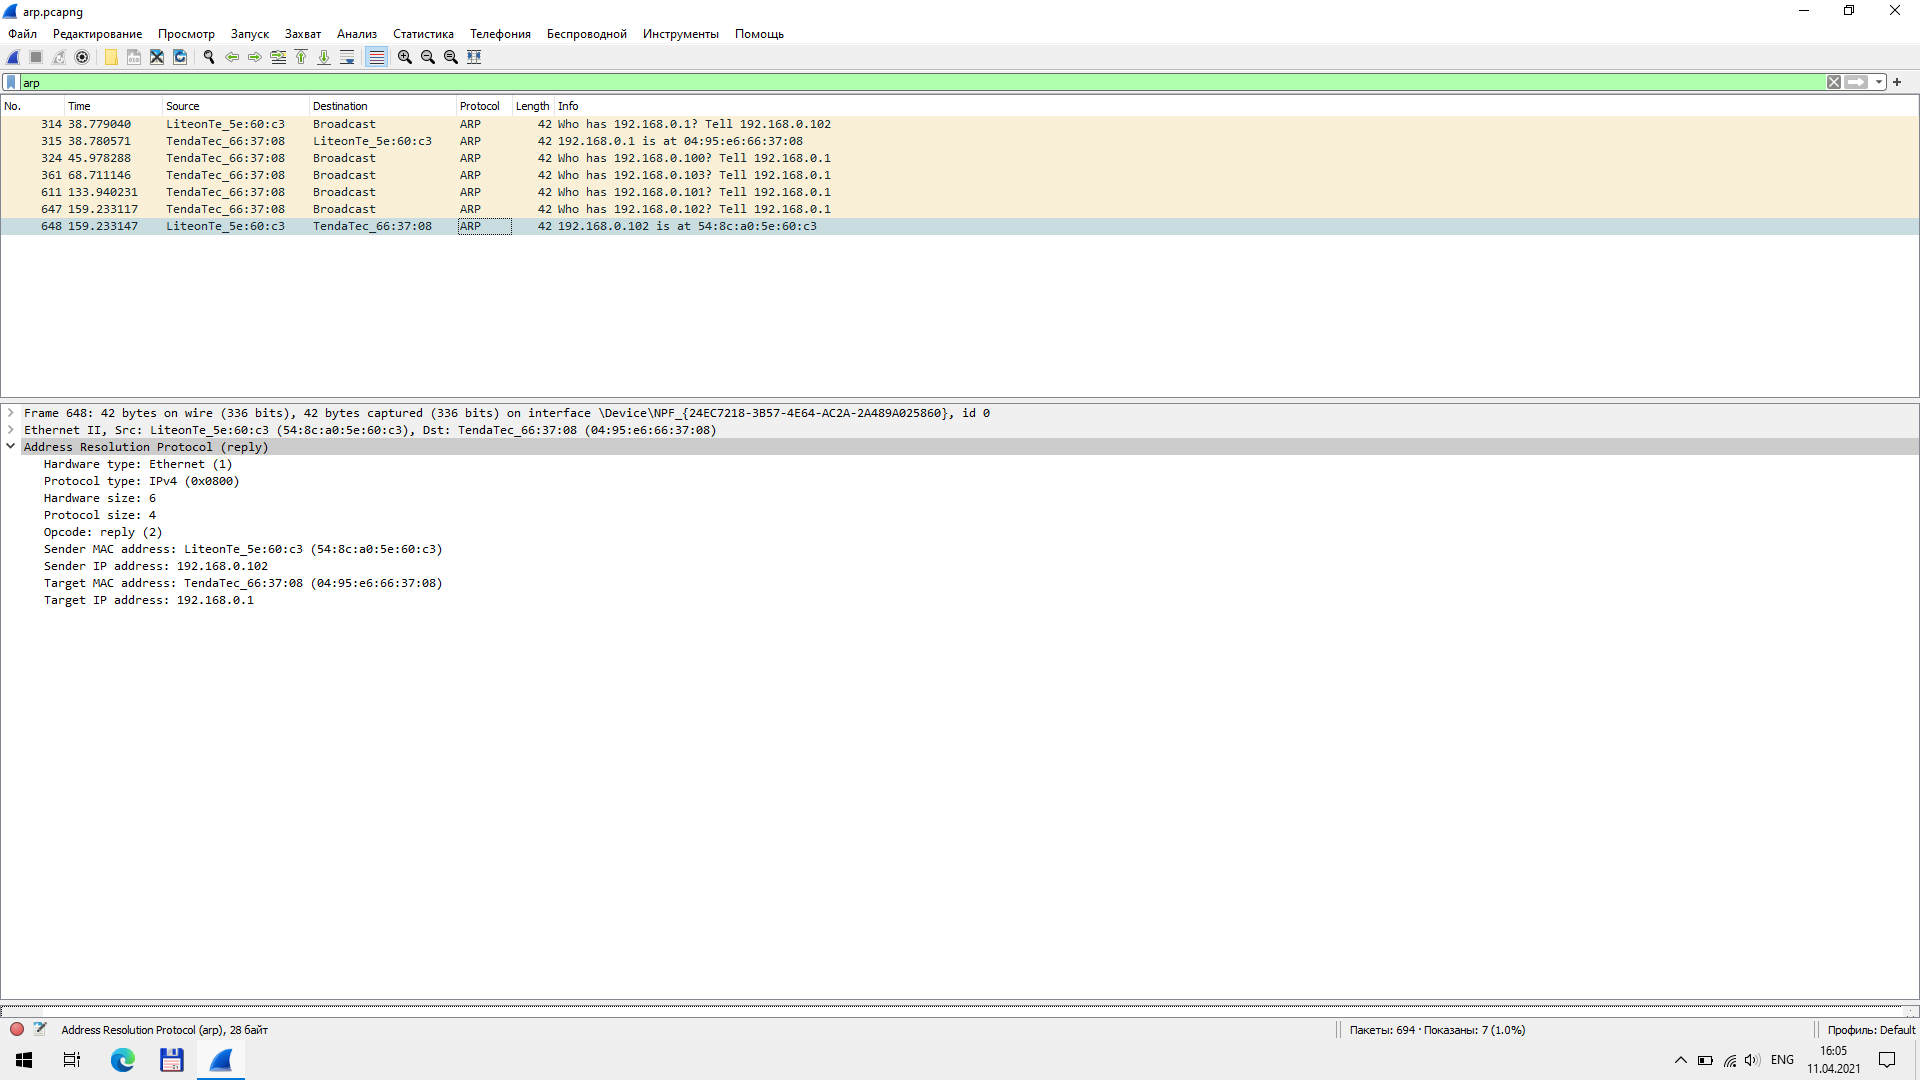
\includegraphics[width=\textwidth]{screenshots/arp_setup_1}

\end{center}

\subsection{Ответы на вопросы}

\subsubsection{}
MAC-адреса устройств в локальной сети: Sender --- адрес отправителя, Target --- получателя.
Если MAC-адрес получателя --- все нули, то это сообщение для всех.
Это идентификаторы сетевых карт всех подключенных к маршрутизатору устройств, включая сам маршрутизатор.
04:95:e6:66:37:08 (192.168.0.1) --- сам маршрутизатор, остальные --- другие компьютеры в сети.

\subsubsection{}
MAC-адреса роутера и компьютера.
Это адреса для обмена канального уровня, IP --- на сетевом (на уровень выше).

\subsubsection{}
Для сообщения своего IP при ответе на ARP-запрос, а также как обратный адрес.
